%----------------------------------------------------------------------------
\chapter{Architektúra}
%----------------------------------------------------------------------------
Az alkalmazás 3 fő részre bontható frontend, backend valamint adatbázis.
E három réteg együttesen felel azért, hogy a felhasználó böngészőn keresztül érkező interrakcióit kezelje és az állapotot tárolja.
%----------------------------------------------------------------------------

\section{Adatbázis séma}
Az adatbázis migrációját nem kellett manuálisan végrehajtanom hála a Prisma-nak. 
A Prisma - amellett, hogy kezeli a migrációkat - egy absztrakciós réteget ad az adatbázisunk és az alkalmazásunk közé.

\begin{figure}[!ht]
  \centering
  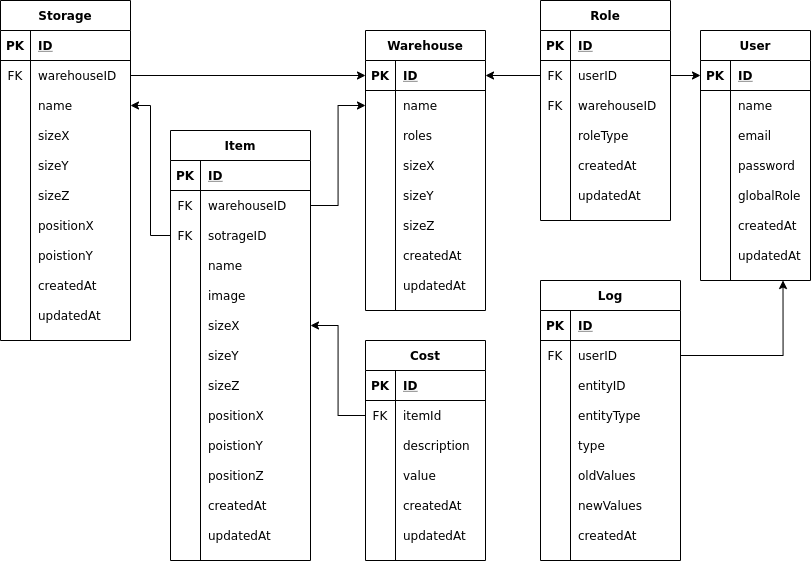
\includegraphics[width=150mm, keepaspectratio]{figures/db.png}
  \caption{Adatbázis séma}
  \label{fig:backend}
\end{figure}

%----------------------------------------------------------------------------

\section{Backend felépítése}
Az alkalmazás üzleti logikáját megvalósító rész (továbbiakban backend) egy NodeJS-re épülő rendszer.
Az alkalmazás egyetlen egy végpontot ajánl a kliensek számára.
A kéréseket egy express server fogadja, a feldolgozásának mikéntjéről pedig egy Apollo server gondoskodik.
Az Apollo server lehetőséget nyújt middelware-ek definiálsára, melyek minden kérés kiszolgálása elött lefutnak.
Erre a lehetőségre épít a GraphQL Shield nevű könyvtár, aminek segítségével minden egyes GraphQL műveletre megadhatünk ahhoz szükséges előfeltételeket egyszerű szabályok segítségével.
Ilyen szabályokkal valósítottam meg a teljes authorizációt és authentikáció ellenörzését.

\begin{figure}[!ht]
  \centering
  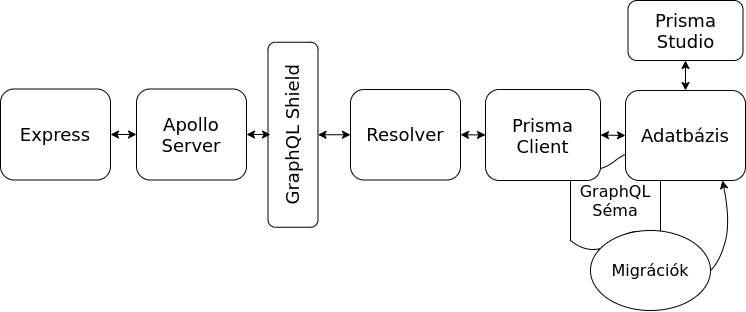
\includegraphics[width=150mm, keepaspectratio]{figures/backend.png}
  \caption{Backend felépítése}
  \label{fig:backend}
\end{figure}

%----------------------------------------------------------------------------

\section{Frontend felépítése}
Ahogy azt a korábbi fejezetekben taglaltam a kliens alkalmazás megvalósításához React azon belül pedig NextJS-t használtam.
%----------------------------------------------------------------------------

\section{A teljes kép}
Frontend ---GraphQL--- backend - DB

\begin{figure}[!ht]
  \centering
  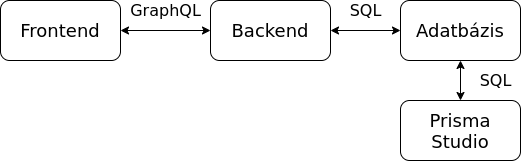
\includegraphics[width=150mm, keepaspectratio]{figures/architecture.png}
  \caption{Teljes alkalmazás felépítése}
  \label{fig:architecture}
\end{figure}